
\subsection*{الف}
مجموعه
$\epsilon - \text{closure}$
استیت‌های
$A$
و
$B$
را مشخص میکنیم.

 تمام استیت هایی که استیت مورد نظر با 
$\epsilon$
به آن میرود و خود استیت را بدست می آوریم.

\lr{$A$ = \{$A$, $D$, $F$, $H$\}
\\
$B$ = \{$B$, $C$\}
\\
}


\subsection*{ب}
برای
NFA
داده شده، یک
DFA
معادل رسم میکنیم.

برای اینکار ابتدا
مجموعه
$\epsilon - \text{closure}$
استیت شروع که در اینجا
$a$
است را یک استیت در نظر میگیریم. سپس استیت هایی که مجموعه 
$\epsilon - \text{closure}$
با 0 و 1 به آن استیت ها میرود را بدست می آوریم.
سپس برای آن استیت ها نیز استیت هایی که با 0 و 1 به آن میروند را بدست می آوریم. این روند را ادامه میدهیم تا به استیت انتهایی و یا تکراری برسیم.

\begin{center}
    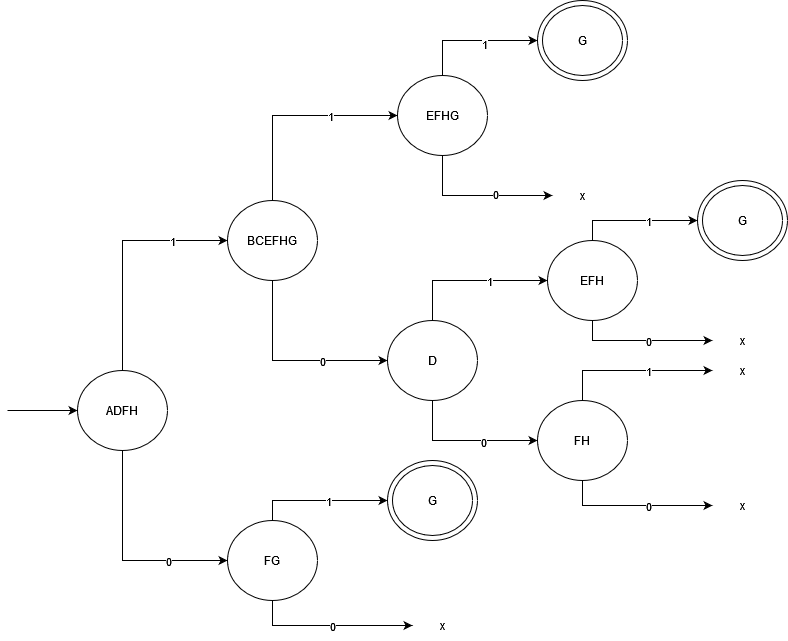
\includegraphics[width = 1\textwidth]{"commons/quiz21.png"}
\end{center}

استیت های تکراری و اضافه را حذف میکنیم
.
NFA 
نهایی به صورت زیر در می آید.
\begin{center}
    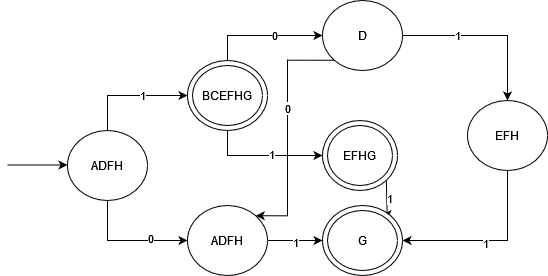
\includegraphics[width = 0.8\textwidth]{"commons/quiz22.png"}
\end{center}